\chapter{Occluder-based Imaging with Real Occluders}

\section{Turning Corners into Cameras}

\subsection{Introduction}

``Turning Corners into Cameras'' is the pithy name for one of the simplest imaging occluder-based imaging techniques---but also one of the most robust, effective, and practical. Although the idea is now years old, I still use it as my first example whenever I want to explain how one might use occluders to image hidden scenes using visible light. And although there's still plenty of work to be done before it could be sold as a product (perhaps to be used in self-driving cars) it is in my own estimation the single likeliest thing in this thesis, or in the subfield of passive visible-light NLoS imaging (that I know of), to be put to practical use in the near future.

So what's the idea? The idea is to use the corner as an edge occluder. In the language of the previous chapter, the ``occluding frame'' is a half-occluding, half-transmitting frame. The transfer matrix that gives you is an upper-triangular matrix. Certainly this matrix will be far from optimal by the standards of the previous chapter! But it's simple and ubiquitous, and if all you're looking for is a 1D reconstruction of the hidden scene, it will work well enough.

This particular type of occluder also has the additional nice property of having, like the pinhole, a particularly recognizable reconstruction algorithm. A pinhole inverts (and blurs) the scene but otherwise doesn't distort it, so that the observation matches the image; an edge occluder integrates the scene, so that if the scene intensity function is $f(x)$, the observation intensity function will be $\int f(x) dx$. That means that in order to reconstruct, all you have to do is take the derivative of your scene with respect to space. This is convenient not only because it means the core algorithm is simple, but also because some cameras already exist which automatically record spatial derivatives at the hardware level~\cite{TODO}.

The headline figure from \emph{Turning Corners into Cameras} explains this idea well; see Fig.~\ref{fig:teaser}. Note how the colors on the floor give us a 1D view of what's in the scene, integrated over space. This is exactly what we expected to see from an edge occluder, given our analysis in the previous chapter. The fact that in this case, the observation plane (i.e. the floor) is perpendicular to the occluder frame (i.e. the wall) is what makes the spatial variation on the floor be a function of angle from the wall, rather than just the $x$-coordinate. (This phenomenon will be one I go into in more detail later.)

\begin{figure}
\begin{center}
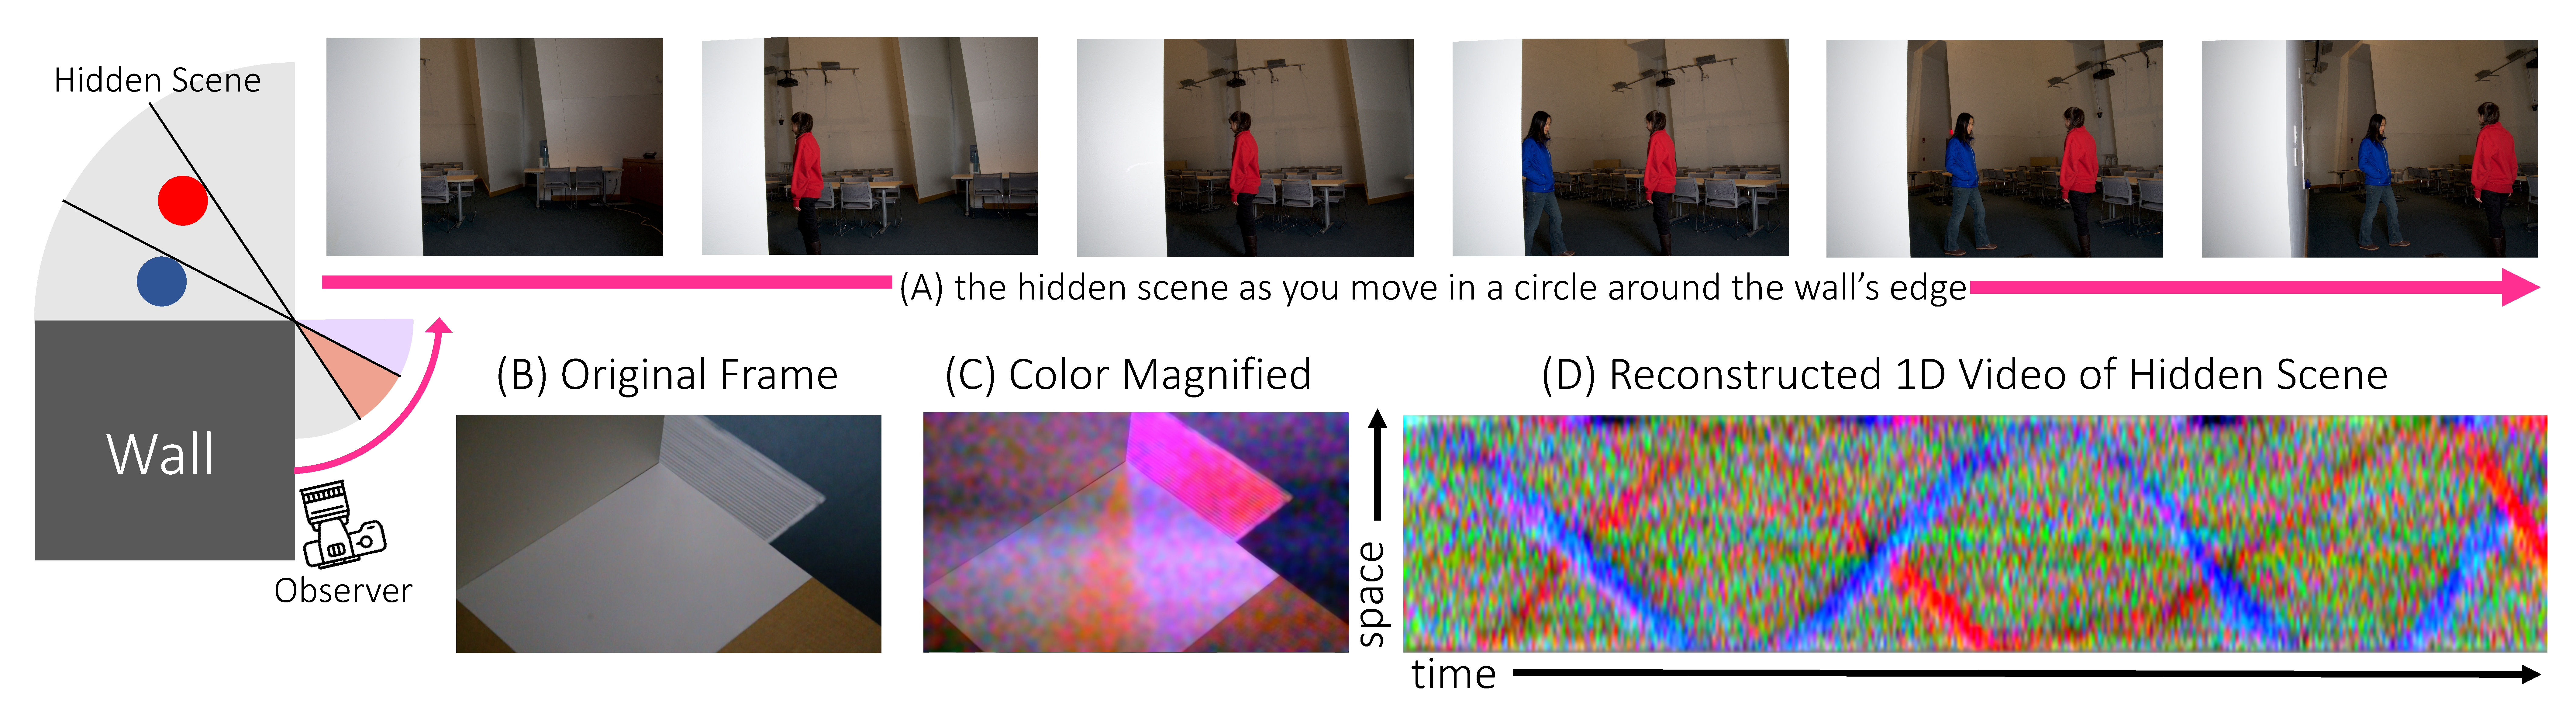
\includegraphics[scale=0.6]{figs/teaser.pdf}
\caption{A method for constructing a 1-D video of an obscured scene. The far left shows a diagram of a typical scenario: two people---one wearing red and the other blue---are hidden from view by a wall. To an observer walking around the occluding edge (along the magenta arrow), light from different parts of the hidden scene becomes visible at different angles (A). Ultimately, this scene information is captured in the intensity and color of light reflected from the corresponding patch of ground near the corner. Although these subtle irradiance variations are invisible to the naked eye (B), they can be extracted and interpreted from a camera position from which the entire obscured scene is hidden from view. Image (C) visualizes these subtle variations in the highlighted corner region. We use temporal frames of these radiance variations on the ground to construct a 1-D video of motion evolution in the hidden scene. Specifically, (D) shows the trajectories over time of hidden red and blue subjects illuminated by a diffuse light in an otherwise dark room. \label{fig:teaser}}
\end{center}
\end{figure}

\subsection{Edge cameras in practice}

\newcommand{\yt}{\mathbf{y}^{(t)}}
\newcommand{\xt}{\mathbf{x}^{(t)}}
%\newcommand{\A}{\mathbf{A}}
%\newcommand{\G}{\mathbf{G}}
%\newcommand{\I}{\mathbf{I}}
\newcommand{\diff}{\mathrm{d}}
\makeatletter   
\newcommand{\Spvek}[2][r]{%
	\gdef\@VORNE{1}
	\left(\hskip-\arraycolsep%
	\begin{array}{#1}\vekSp@lten{#2}\end{array}%
	\hskip-\arraycolsep\right)}

\def\vekSp@lten#1{\xvekSp@lten#1;vekL@stLine;}
\def\vekL@stLine{vekL@stLine}
\def\xvekSp@lten#1;{\def\temp{#1}%
	\ifx\temp\vekL@stLine
	\else
	\ifnum\@VORNE=1\gdef\@VORNE{0}
	\else\@arraycr\fi%
	#1%
	\expandafter\xvekSp@lten
	\fi}
\makeatother

An edge camera system consists of four components: the visible and hidden scenes, the occluding edge,
and the ground, which reflects light from both scenes. We refer to the (ground) plane perpendicular to the occluding edge as the {\it observation plane}.
%An example
%system is shown in Figure~\ref{fig:corner_diagram}. Here, a moving red object and a moving blue object are  obscured by the corner of a building. 
By analyzing subtle variations in the penumbra at the base of an edge, we are able to deduce a hidden subject's pattern of motion.

The reflected light from a surface at point $p$ is a function of the incoming light $L'_i$ as well as the surface's albedo $ a $ and BRDF 
%bidirectional reflectance distribution function (BRDF) 
$\beta$. Specifically, 
\begin{align}
L_o'(p,\hat{v}_o) = a(p) \int L'_i(p,\hat{v}_i) \, \beta( \hat{v}_i, \hat{v}_o, \hat{n} ) \,\gamma(\hat{v}_i, \hat{n}) \, \diff \hat{v}_i,
\label{eq:first_equation}
\end{align}
where $\hat{v}_i$ and $\hat{v}_o$ denote the incoming and outgoing unit vectors of light at position $p = (r,\theta)$, respectively, and $\gamma(\hat{v}_i, \hat{n}) = \frac{ \hat{v}_i \cdot \hat{n} }{  \hat{v}_i  \hat{n} }$.
%for the computation of the irradiance. 
We parameterize $p$ in polar coordinates, with the origin centered at the occluding edge and $\theta=0$ corresponding to the angle parallel to the wall coming from the corner (refer to Fig.~\ref{fig:transfermtx}). For simplicity, we assume the observation plane is Lambertian, and that the visible and hidden scene are modeled as light emitted from a large celestial sphere, parameterized by right ascension $\alpha$ and declination $\delta$. Under these assumptions, we simplify \eqref{eq:first_equation}: 
%$\beta=1$ and $L_i$ and $\theta_o$ are equivalent for each location, $\ell$: 
%\begin{align}
%L_o(\ell) = \alpha(\ell) \int L_i(\hat{v}_i)  \gamma(\hat{v}_i)  d \hat{v}_i
%\end{align}
\begin{align}
L'_o(r,\theta) &= a(r,\theta) \int_{\alpha=0}^{2 \pi} \int_{\delta=0}^{\pi/2} L_i(\alpha, \delta) \, \diff \alpha \, \diff \delta 
\end{align}
where $L_i(\alpha, \delta) = L'_i(\alpha, \delta)  \gamma(\alpha, \delta)$. Furthermore, since the occluding edge blocks light from $[\pi+\theta, 2 \pi]$ at radial line $\theta$, 
\begin{align}
L'_o(r,\theta) & = a(r,\theta) \left[ L_v + \int_{\phi=0}^{\theta}  L_h(\phi)\, \diff \phi \right]
\label{eq:finalfulleq}
\end{align}
%\begin{align}
%\notag L_o(r,\theta) &= a(r,\theta) \int_{\alpha=0}^{\pi + \theta} \int_{\delta=0}^{\pi/2} L_i(\alpha, \delta)  d \alpha d \delta \\
%& = a(r,\theta) \left[ L_v + \int_{\phi=0}^{\theta}  L_h(\phi) d\phi \right]
%\end{align}
for {\small $L_v = \int_{\alpha=0}^{\pi} \int_{\delta=0}^{\pi/2} L_i(\alpha, \delta) \, \diff \alpha\, \diff \delta$} and {\small $L_h(\phi) = \int_{\delta=0}^{\pi/2} L_i(\pi + \phi, \delta)\, \diff \delta$}. By inspecting \eqref{eq:finalfulleq} we can see that the intensity of light on the penumbra is explained by a constant term, $L_v$, 
which is the contribution due to light visible to the observer, and a varying angle dependent term which integrates the light in the hidden scene, $L_h$. 
For instance, a radial line at $\theta=0$ only integrates the light from the scene visible to the observer, while the radial line $\theta=\pi/2$ reflects the integral of light over the entire visible and hidden scenes.  




\begin{figure}[tb]
\centering
%\subfigure[Constructing the Transfer Matrix $\mathbf{A}$]
\vspace{-1em}
{\includegraphics[width=1\linewidth]{figs/transfermtx2.pdf}}
%\subfigure[estimation Gain Image]{\includegraphics[width=0.45\linewidth]{figs/kalman.pdf}}
\vspace{-.3in}
\caption{\label{fig:transfermtx} 
%The relationship between observations $\yt$ and the hidden scene $\xt$. 
In (A), the transfer matrix, $\A$, is shown for a toy situation in which observations lie along circles around the edge. %Each of these observations sees one more angular component of the hidden scene than its neighbor, so 
In this case, $\A$ would simply be a repeated lower triangular matrix. (B) contains an example estimation gain image, which describes the matrix operation performed on observations $\yt$ to estimate $\xt$. As predicted, the image indicates that we are essentially performing an angular derivative in recovering a frame of the 1-D video.}
\vspace{-1em}
\end{figure}


Then, the derivative of the observed penumbra 
%the Fundamental Theorem of Calculus tells us that 
recovers the 1-D angular projection of the hidden scene: 
\begin{align}
\frac{\diff}{\diff\theta} L'_o(r,\theta) &= a(r,\theta) \,  L_h(\phi) .
\end{align}

But what happens if someone walks into the hidden scene at time $t$, changing $L^{0}_h(\phi)$ to $L^{t}_h(\phi)$? In this case, the spatial derivative of the temporal difference encodes the angular change in lighting: 
\begin{equation}
\frac{d}{d \theta} \left[ L_o'^{t}(r,\theta) - L_o'^{0}(r,\theta) \right] = a(r,\theta) \left[ L^{t}_h(\theta) -  L^{0}_h(\theta)  \right]
\label{eq:subtract_out}
\end{equation}

%% log stuff
%\begin{align}
%& \log( L_o^{t}(r,\theta) ) - log( L_o^{0}(r,\theta) )  = \\ 
%& \log( A(r,\theta) \left[ L_v + \int_{\phi=0}^{\theta}  L_h(\phi) d\phi \right] ) - log( A(r,\theta) \left[ L_v + \int_{\phi=0}^{\theta}  L_h(\phi) d\phi \right] ) \\
%& =  \log( \left[ L_v + \int_{\phi=0}^{\theta}  L_h(\phi) d\phi \right] ) - log( \left[ L_v + \int_{\phi=0}^{\theta}  L_h(\phi) d\phi \right] ) 
%\end{align}

\noindent{In other words, the angular derivative of the penumbra's difference from the reference frame is a signal that indicates the angular change in the hidden scene over time. In practice, we obtain good results  assuming $a(r,\theta) = 1$ and using the cameras' native encoded intensity values. 
%(assuming, for simplicity, a constant albedo on the observation plane). 
%In Section~\ref{sec:methods_edges2} we explain the procedure we use to reconstruct a one-dimensional angular image of the changes in the hidden scene from the penumbra. 
}


\vspace{-.1in}
\subsection{Method}
\label{sec:methods_edges2}

Using a video recording of the observation plane, we  generate a 1-D video indicating the changes in a hidden scene over time. These 1-D angular projections of the hidden scene viewed over many time-steps reveal
the trajectory of a moving object behind the occluding edge.

\vspace{-.1in}
\paragraph{Likelihood: } At each time $t$, we relate the observed $M$-pixels on the projection plane, $\yt$, to the 1-D angular projection of the hidden scene, $L_h^{(t)} (\phi)$.
%In order to recover the hidden scene at time $t$ 
We formulate a discrete approximation to our edge camera system by describing the continuous image $L_h^{(t)} (\phi)$ using $N$ terms, $\xt$.
%Please refer to Section~\ref{sec:impdetail} for more details. 
The observations $\yt$ then relate to the unknown parameters $\xt$ and $L_v^{(t)}$ by a linear matrix operation:
\begin{align}
 \notag   \yt = L_v^{(t)} + \A\xt + \mathbf{w}^{(t)},\qquad
    \mathbf{w}^{(t)} \sim \mathcal{N}(0, \lambda^2\mathbf{I}),
\end{align}
%: $x[n]$ for $\phi = \frac{\pi n}{2N} + \frac{\pi}{4N} $ for $n=0,...,N$. 
%$n=\frac{\pi}{4N},\frac{3\pi}{4N}, ...,\frac{\pi}{2} - \frac{\pi}{4N}$. 
%WE ARE IGNORING ALBEDO HERE
%We formalize our problem with Figure~\ref{fig:edgecam_defs}
%\begin{figure}
%    \centering
%    \includegraphics[width=0.5\linewidth]%{edgecam_defs.png}
%    \caption{\label{fig:edgecam_defs} A top-down view of an edge camera. We label the
%        observations $\yt$ and the 1-D angular projection of the hidden scene $L_h^{(t)} (\phi) $
%        as we will refer to them throughout the paper.}
%\end{figure}
%At each timestep $t$, we can relate the light intensities observed on our projection plane,
%$\yt$, and the 1-D angular projection of the hidden scene, $\xt$ with a linear relation
where the $M \times N$ matrix $\A$ is defined by the geometry of the system. More
explicitly, each row $m$ of $\A$ integrates the portion of the hidden scene
visible from observation $m$, $\yt_m$. In the simplified case of observations that lie on a circle around the occluding edge,
%with observations taken from a constant-albedo observation plane, 
$\A$ would simply be a constant lower-triangular matrix;
%, and its inverse would be a difference matrix.
see Fig.~\ref{fig:transfermtx}A. 



Let $\widetilde{\A}$ be the column augmented matrix $ \left[ \mathbf{1} \hspace{0.05in} \A \right]$. We can then express the likelihood of an observation given $\xt$ and $L_v^{(t)}$ as:
\begin{equation}
    p(\yt|\xt, L_v^{(t)} ) = \mathcal{N} \left(\widetilde{\A} \left[ L_v^{(t)} \hspace{0.05in} {\mathbf{x}}^{(t)T} \right]^T, \lambda^2\I \right).
\end{equation}

\vspace{-.1in}
\paragraph{Prior: }
%The signal we are trying to extract is very small relative to the dynamic range of a typical camera sensor. 
%\katie{is that the correct use of dynamic range?}
The signal we are trying to extract is very small relative to the total light intensity on the observation plane.
%We perform inference on $\xt$ using various models. 
Therefore, to improve the quality of results, we enforce spatial
%and temporal 
smoothness of $\xt$. 
%Since we expect the hidden scene to have spatial coherence, 
We use a simple L2 smoothness regularization 
over adjacent parameters in $\xt$. This corresponds, for a gradient matrix $\G$, to using the prior
\begin{align}
% \notag   p(\xt) &\propto \prod_{n=1}^{N-1} \exp \left[ -\frac{1}{2\sigma^2}  (\xt[n] - \xt[n-1])^T(\xt[n] - \xt[n-1]) \right] \\
  \notag   p(\xt) &\propto \prod_{n=1}^{N-1} \exp \left[ -\frac{1}{2\sigma^2}  \Vert  \xt[n] - \xt[n-1] \Vert_2 ^2 \right] \\
          % &= \exp \left[ -\frac{1}{2\sigma^2} (\xt)^T \G^T\G \xt \right] \\
           &= \mathcal{N}(0, \sigma^{2} (\G^T \G)^{-1} ).
\end{align}

%\noindent{for gradient matrix $\G$.}

\vspace{-.1in}
\paragraph{Inference: }

We seek a maximum a posteriori (MAP) estimate of the hidden image coefficients, $\xt$, given $M$ observations, $\yt$, measured by the camera. By combining the defined Gaussian likelihood and prior distributions, we obtain a Gaussian posterior distribution of $\xt$ and $L_v^{(t)}$, 

\begin{align}
%p(\xt|\yt) & \propto p(\yt|\xt) p(\xt) = \mathcal{N}_{x} ( \hat{\bf{x}}^{(t)}, \Sigma^{(t)} ) \\
\notag p(\xt, L_v^{(t)} |\yt) & = \mathcal{N} \left( \left[ \hat{L}_v^{(t)} \hspace{0.05in} {\hat{\mathbf{x}}}^{(t)T} \right]^T , \Sigma^{(t)} \right) \\
\notag \Sigma^{(t)} &= \left[\lambda^{-2}\widetilde{\A}^T\widetilde{\A} + \sigma^{-2} \Spvek{ \mathbf{0} \hspace{0.35in} \mathbf{0} ; \mathbf{0} \hspace{0.1in} \G^T\G } \right]^{-1} \\
%\hat{\bf{x}}^{(t)} &= (G^TG)^{-1} A^T ( \lambda {\bf I} +   A   (G^TG)^{-1} A^T)^{-1} y \\ 
%\Spvek{ \hat{L}_v^{(t)}; \hat{\bf{x}}^{(t)} } =
\left[ \hat{L}_v^{(t)} \hspace{0.05in} {\hat{\mathbf{x}}}^{(t)T} \right]^T &= \Sigma^{(t)}
            \lambda^{-2}\widetilde{\A}^T\yt  
\end{align}
where the maximum a posteriori estimate is  given by $\hat{\bf{x}}^{(t)}$.

To better understand the operation that is being performed to obtain the 1-D reconstruction, we visualize each row of the matrix $\Sigma^{(t)}\lambda^{-2}\widetilde{\A}^T $. We refer to each reshaped row of this matrix as the {\it estimation gain image}. An example estimation gain image is shown in Fig.~\ref{fig:transfermtx}B. Note that, as expected, the matrix operation is computing an angular derivative over the observation plane. 
%\begin{equation}
%    \xt = \left[\lambda^{-1}\A^T\A + \sigma^{-2}\G^T\G \right]^{-1}
%            \left[\lambda^{-1}\A^T\yt \right].
%\end{equation}

\begin{figure*}[tb]
\centering
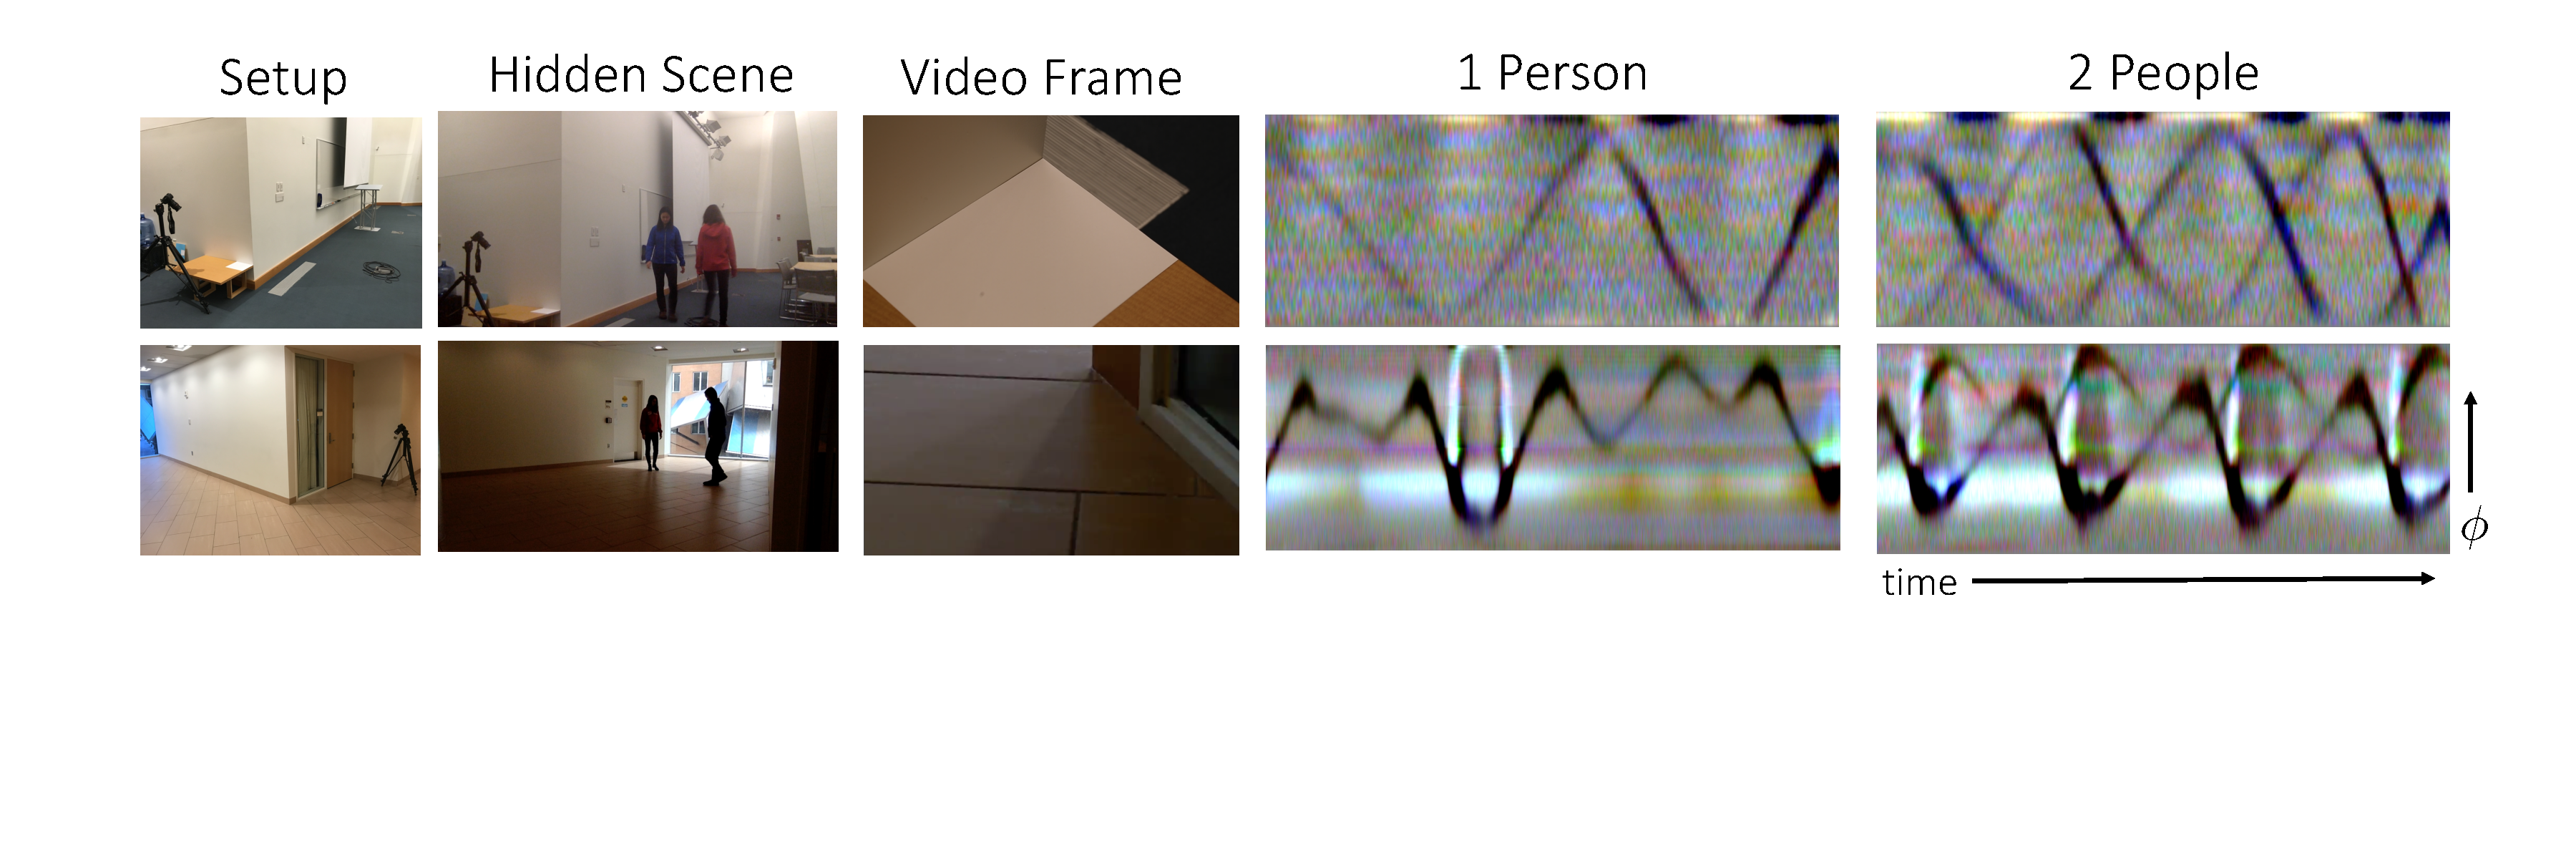
\includegraphics[width=\linewidth]
{figs/indoorfigure.pdf}
\vspace{-1in}
\caption{\label{fig:indoorfigure} One-dimensional reconstructed videos of indoor, hidden scenes. Results are shown as space-time images for sequences where one or two people were walking behind the corner. In these reconstructions, the angular position of a person, as well as the number of people, can be clearly identified. Bright line artifacts are caused by additional shadows appearing on the penumbra.
}
\vspace{-.2in}
\end{figure*}

\begin{figure*}[tb]
\centering
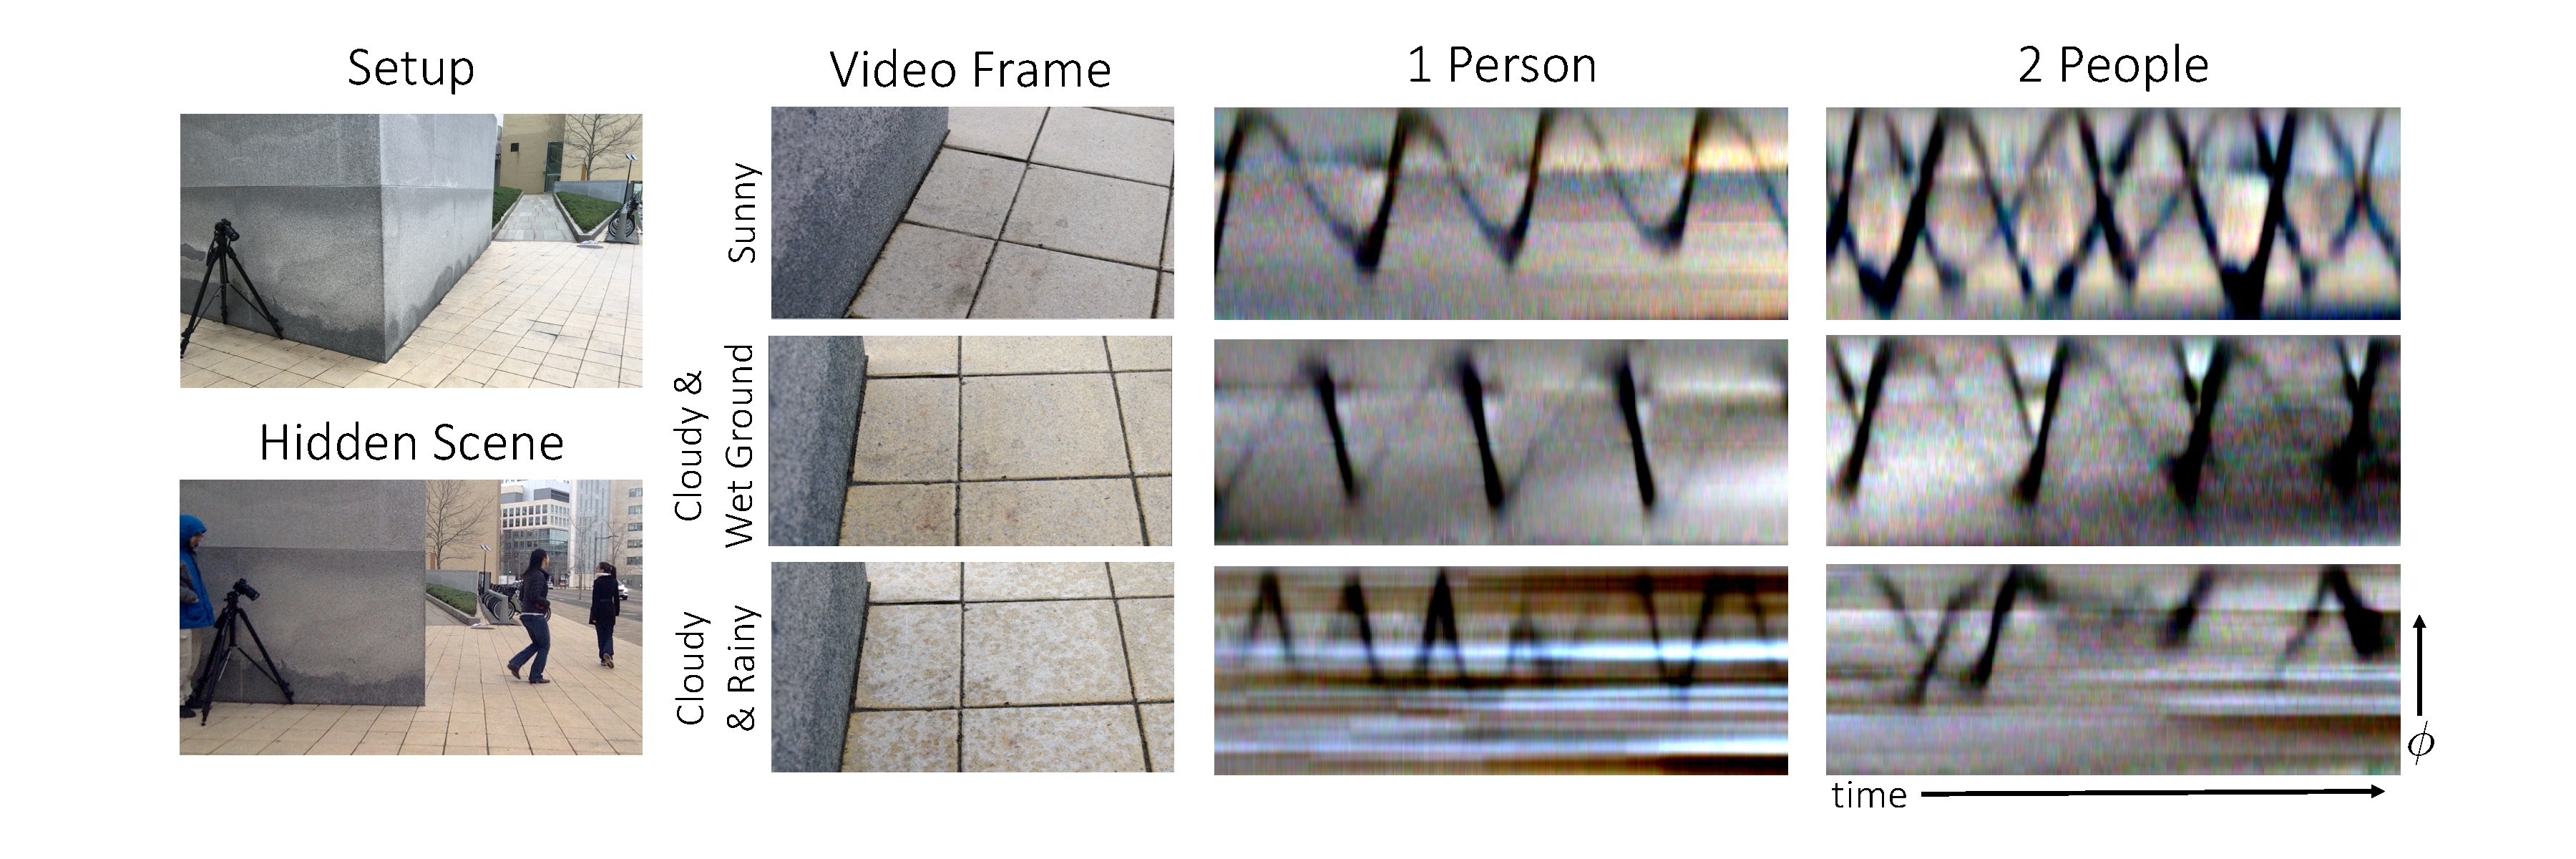
\includegraphics[width=\linewidth]{figs/outdoorfigure4.pdf}
\vspace{-.4in}
\caption{\label{fig:outdoorfigure4}  1-D reconstructed videos of a common outdoor, hidden scene under various weather conditions. Results are shown as space-time images. The last row shows results from sequences taken while it was beginning to rain. Although artifacts appear due to the appearing raindrops, motion trajectories can be identified in all reconstructions.}
\end{figure*}


\begin{figure*}[tb]
\centering
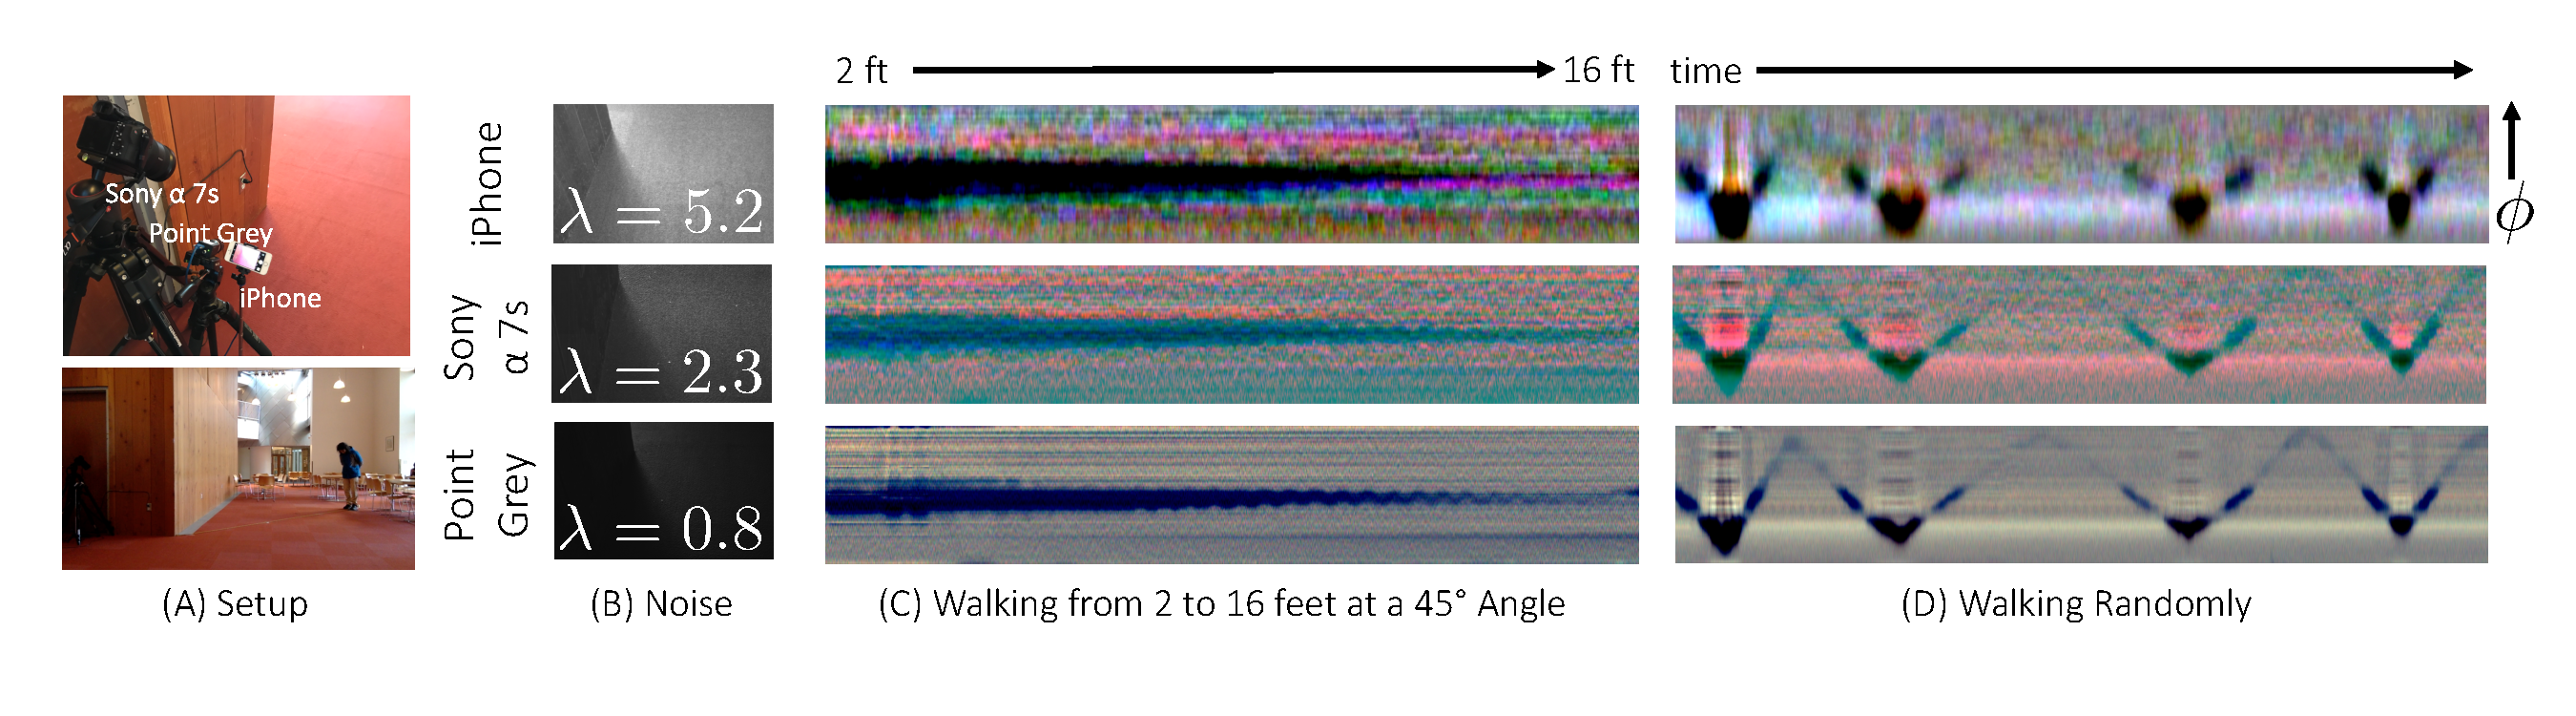
\includegraphics[width=1\linewidth]{figs/multicamera2.pdf}
\vspace{-.5in}
\caption{The result of using different cameras on the reconstruction of the same sequence in an indoor setting. Three different 8-bit cameras (an iPhone 5s, a Sony Alpha 7s SLR, and an uncompressed RGB Point Grey) simultaneously recorded the carpeted floor. Each camera introduced a different level of per-pixel sensor noise. 
The estimated standard deviation of sensor noise, $\lambda$, is shown in (B). 
%The median sensor noise, $\lambda$, for each camera is shown in (B) along with a per-pixel image of the noise's standard deviation.
% The standard deviation of noise for each camera is shown in (B) along with the median value. 
%The median standard deviation of noise for the iPhone, Sony $\alpha$ 7s, and Point Grey are 5.2, 2.3, and 0.8, respectively. 
%Here, white indicates a standard deviation of 7 for an 8-bit image (. 
We compare the quality of two sequences in (C) and (D).  In (C), we have reconstructed a video from a sequence of a single person walking directly away from the corner from 2 to 16 feet at a 45 degree angle from the occluded wall. This experiment helps to illustrate how signal strength varies with distance from the corner. In (D), we have done a reconstruction of a single person walking in a random pattern. \label{fig:multicamera}}
\vspace{-.2in}
\end{figure*}

\vspace{-.1in}
\subsubsection{Implementation Details}
\label{sec:impdetail}

\vspace{-.1in}
\paragraph{Rectification:} All of our analysis thus far has assumed we are observing the floor
%at a 90 degree angle. 
parallel to the occluding edge. %its normal direction.
However, in most situations, the camera will be observing the projection plane at an angle. In order to make the construction of the matrix $\A$ easier, we begin by rectifying our images using a homography. 
%In particular, we compute a homography that transforms our image such that a circle on the projection plane in pixel space corresponds to a circle in absolute space. 
In these results, we assume the ground is perpendicular to the occluding edge, and estimate the homography using either a calibration grid or regular patterns, such as tiles, that naturally appear on the ground. Alternatively, a known camera calibration could be used. 

%\vspace{-.1in}
%\paragraph{Image Parameterization:} The 1-D image $L_h^{(t)} (\phi)$ we wish to recover is defined over the continuous space of angular coordinates $\phi=[0,\pi/2]$.
%Rather than simply assuming a discretized image of point
%sources for reconstruction, we instead parameterize a continuous image using $N$ terms, $\xt$. We approximate $L_h^{(t)} (\phi)$ as a series of scaled and shifted triangle functions with width $\frac{\pi}{N}$. This representation linearly interpolates between specified centers, and the contribution of each parameter $\xt_n$ to each $\yt_m$ 
%can be easily calculated.

%\katie{I THINK WE ARE OFF BY ONE HERE}
%\begin{align}
%L_h^{(t)} (\phi) \approx \sum_{n=0}^{N-1} \xt [n] \max \left(1 - \frac{\left| \frac{\pi (2 n + 1) }{4N}  - \phi \right|}{\pi/2N}, 0 \right)
%\end{align}

\vspace{-.1in}
\paragraph{Background Subtraction: }

Since we are interested in identifying temporal differences in a hidden scene due to a moving subject, we must
%Focusing on the differences allows us to more easily tease out the signal corresponding to a hidden target. 
remove the effect of the scene's background illumination.  Although this could be accomplished by first subtracting a background frame, $L_o^0$, taken without the subject, we avoid requiring the availability of such a frame. Instead,  we assume the subject's motion is roughly uniform over the video, and use the video's mean image in lieu of a true background frame. 

\vspace{-.1in}
\paragraph{Temporal Smoothness: }

In addition to spatial smoothness we could also impose temporal smoothness on our MAP estimate. $\hat{\bf{x}}^{(t)}$. This helps to further regularize our result, at the cost of some temporal blurring.
However, to emphasis the coherence among results, we do not impose this additional constraint. Each 1-D image, $\xt$, that we show is independently computed.
%and is the result of averaging together ten frames. \katie{check that it is still ten frames at submission time.}
Results obtained with temporal smoothness constraints are shown in the supplemental material. 

%\katie{Haven't yet mentioned the temporal averaging}

\vspace{-.1in}
\paragraph{Parameter Selection: }
The noise parameter $\lambda^2$ is set for each video as the median variance of estimated sensor noise. The spatial smoothness parameter, $\sigma$, is set to 0.1 for all results.


\vspace{-.1in}
\subsection{Experiments and Results}


Our algorithm reconstructs a 1-D video of a hidden scene from behind an occluding edge, allowing users to track the motions of obscured, moving objects. 
%As we are interested in reconstructing a 1-D projection of the hidden scene over time,
In all results shown, the subject was not visible to an observer at the camera. 


We present results using space-time images. These images contain curves that indicate the angular trajectories of moving people. All results, unless specified otherwise, were generated from standard, compressed video taken with a SLR camera. Please refer to the supplemental video for full sequences and additional results.

\subsubsection{Environments}

We show several applications of our algorithm in various indoor and outdoor environments. For each environment, we show the reconstructions obtained when one or two people were moving in the hidden scene. 
%As predicted, our results suggest that the larger the contrast between the background illumination of the hidden scene and the moving subject, the better the reconstructed 1-D video.  

\vspace{-.1in}
\paragraph{Indoor:}
In Fig.~\ref{fig:teaser} we show a result obtained from a video recorded in a mostly dark room. A large diffuse light illuminated two hidden subjects wearing red and blue clothing. As the subjects walked around the room, their clothing reflected light, allowing us to reconstruct a 1-D video of colored trajectories. As correctly reflected in our constructed video, the subject in blue occludes the subject in red three times before the subject in red becomes the occluder. 
% compared to their enviroment

Fig.~\ref{fig:indoorfigure} shows additional examples of 1-D videos recovered from indoor edge cameras. In these sequences, 
the environment was well-lit. The subjects
occluded the bright ambient light, resulting in the reconstruction's dark trajectory. Note that in all the reconstructions, it is possible to count the number of people in the hidden scene, and to recover important information such as their angular size and speed, and the characteristics of their motion.
%about their movement, such as whether they are moving randomly or periodically.

\vspace{-.1in}
\paragraph{Outdoor: }
In Fig.~\ref{fig:outdoorfigure4} we show the results of a number of videos taken at a common outdoor location, but in different weather conditions. The top sequences were recorded during a sunny day, while the bottom two sequences were recorded while it was cloudy. Additionally, in the bottom sequence, raindrops appeared on the ground {\it during} recording, while in the middle sequence the ground was fully saturated with water.  
%middle sequence the ground was fully saturated while sequence 2 was recorded while it was cloudy and rainy. 
Although the raindrops cause artifacts in the reconstructed space-time images, you can still discern the trajectory of people hidden behind the wall. 






%\begin{figure}
%\centering
%\includegraphics[width=\linewidth]{figs/outdoorfigure3.pdf}
%\caption{\label{fig:outdoorfigure3} }
%\end{figure}


%\begin{figure}
%    \centering
%    \includegraphics[width=\linewidth]{teaser_diagram.png}
%    \caption{\label{fig:teaser} Teaser placeholder}
%\end{figure}

%\begin{figure}
%\centering
%\includegraphics[width=\linewidth]{outdoor_sunny_tmp.png}
%\caption{\label{fig:outdoor_sunny} Outdoor sunny, one and two people walking in circles.}
%\end{figure}

\vspace{-.1in}
\subsubsection{Video Quality: } In all experiments shown thus far we have used standard, compressed video captured using a SLR camera.
%a Sony Alpha 7s or a Canon 6D SLR camera. 
%In our calculations, we generally assumed i.i.d. Gaussian noise. 
However, 
%because the cameras automatically compress captured images, 
video compression can create large, correlated noise that may affect our signal. 
%as we are interested in extracting very small signals, 
We have explored the effect video quality has on results. To do this, we filmed a common scene using 3 different cameras: an iPhone 5s, a Sony Alpha 7s SLR, and a uncompressed RGB Point Grey. Fig.~\ref{fig:multicamera} shows the results of this experiment assuming different levels of i.i.d. noise. Each resulting 1-D image was reconstructed from a single frame. 
The cell phone camera's compressed videos resulted in the noisiest reconstructions, but even those results still capture key features of the subject's path.
%Unsurprisingly, the iPhone resulted in the noisiest reconstructions, but even those results still capture key features of the subject's path.


%\katie{Mention Gamma}

%In the supplemental materials, we analyze the effect of these compression techniques on the noise we see.
% TODO supplemental
%EFFECT OF COMPRESSION ON CORRELATIONS IN THE NOISE SHOWN IN SUPPLEMENTAL.


\vspace{-.1in}
\subsubsection{Velocity Estimation} 

The derivative of a person's trajectory over time, $\phi^{(t)}$, indicates their angular velocity. Fig.~\ref{fig:angularvelocity} shows an example of the estimated angular velocity obtained from a single edge camera when the hidden subject was walking roughly in a circle. Note that the person's angular size and speed are both larger when the person is closer to the corner. Such cues can help approximate the subject's 2-D position over time. 
%higher when they are closer to the corner, assuming their speed is approximately constant over time. 
%This feature could potentially be used to help approximate the subject's 2-D position over time. 


\begin{figure}[!htb]
\centering
\includegraphics[width=0.75\linewidth]{figs/angularvelocity.pdf}
\caption{A subject's reconstructed angular velocity relative to the corner as a function of time. In this sequence, a person was walking in circles far from the corner. \label{fig:angularvelocity} }
\vspace{-.2in}
\end{figure}


%\vspace{-.1in}
\section{Stereo Edge Cameras \label{sec:methods_stereo}}

%In Fig.~\ref{fig:stereodiagram2} we show
%\begin{figure}
%    \centering
%    \includegraphics[width=1\linewidth]{stereodiagram2.pdf}
%    \caption{\label{fig:stereodiagram2} Stereo Diagram}
%\end{figure}



Although the width of a track recovered in the method of the previous section can give some indication of a hidden person's relative range, more accurate methods are possible by exploiting adjacent edges.  In, for example, a hidden scene behind a doorway, the pair of vertical doorway edges yield a pair of corner cameras that inform us about the hidden scene. By treating the observation plane at the base of each edge as a camera, we can obtain stereo 1-D images that we can then use to triangulate the absolute position of a subject over time. 




%this figure shows how to infer its 2-D position from the discrepancy in the angular location recovered from each edge camera.

%We can therefore use the parallax change between these edge cameras to triangulate the position of a hidden object over time. 

%\vspace{-.1in}
\subsection{Method}


A single edge camera allows us to reconstruct
a $90^{\circ}$ angular image of an occluded scene. We now consider a system composed
of four edge cameras, such as an open doorway, as illustrated in Fig.~\ref{fig:stereodiagram1}. Each side of the doorway contains two adjacent edge cameras, whose reconstructions
together create a $180^{\circ}$ view of the hidden scene. 

\begin{figure}[tb]
\centering
\includegraphics[width=0.7\linewidth]{figures/stereodiagram_small.pdf}
\vspace{-.2in}
\caption{The four edges of a doorway contain penumbras that can be used to reconstruct a $180^{\circ}$ view of a hidden scene. The top diagram indicates the penumbras and the corresponding region they describe. 
%how the labeled penumbras correspond to regions of the room.
Parallax occurs in the reconstructions from the left and right wall. This can be seen in the bottom reconstruction of two people hidden behind a doorway. Numbers/colors indicate the penumbras used for each $90^{\circ}$ space-time image.
\label{fig:stereodiagram1}}
\vspace{-.2in}
\end{figure}

The two sides of the doorway provide two views of the same hidden scene, but from different positions. This causes an offset in the projected angular position of the same person (see Fig.~\ref{fig:stereodiagram2}).
Our aim is to use this angular parallax to triangulate the location of a hidden person over time. 
Assume we are observing the base of a doorway, with walls of width $w$ separated by a distance $B$. 
A hidden person will introduce an intensity change on the left and right wall penumbras at angles of $\phi^{(t)}_L$ and $\phi^{(t)}_R$, respectively. 
%A hidden person will introduce an intensity change at an angle $\phi^{(t)}_L$ on the left side of the doorway and $\phi^{(t)}_R$ on the right side. 
%cause a trajectory centered at location $\phi^{(t)}_L$ on the 180 degree reconstruction from the left side of the doorway, and  $\phi^{(t)}_R$ on the right side. 
From this correspondence, we can triangulate their 2-D location.




%\begin{figure}
 %   \centering
%    \includegraphics[width=1\linewidth]{stereodiagram1.pdf}
 %   \caption{\label{fig:stereodiagram1} Stereo Diagram}
%\end{figure}



%More specifically, we can triangulate the position of hidden elements by matching
%the angles they occur at in the right and left 1-D reconstructions of the scene.
%We consider the scenario given in Fig.~\ref{fig:stereocamdiagram}.


\begin{align}
    P_{z}^{(t)} &= \frac{B - \eta^{(t)} }{\cot{\phi_L^{(t)} } + \cot{\phi_R^{(t)}}} \\
    P_{x}^{(t)} &= P_{z}^{(t)} \cot{\phi_L^{(t)}} 
    \label{eq:stereo_xy} \\
       \eta^{(t)} &=
    \begin{cases} 
      w \cot( \phi_R ) & P_x \leq 0 \\
      0 & 0\leq P_x\leq B \\
       w \cot (\phi_L) & P_x \geq B 
   \end{cases}
\end{align}



\noindent{where $ ( P_x, P_z) $ are the $x$- and $z$-coordinate of the person. We define the top corner of the left doorway, corner 1 in Fig.~\ref{fig:stereodiagram1}, as % corresponds to 
$(P_x, P_z) = (0,0)$. }

%Let the top left corner of the doorway be the origin of our system. The
%$y$ coordinate of our object is its depth.  
%The hidden person occurs at angle $\theta_L$ in the left side reconstruction,
%and at angle $\theta_R$ in the right side reconstruction. Then, given a known
%baseline $b$, we triangulate the hidden person's position as



Assuming the wall is sufficiently thin compared to the depth of moving objects in the hidden scene, the $\eta^{(t)}$ term can be ignored. In this case the relative position of the person can be reconstructed without any knowledge of the absolute geometry of the doorway (e.g. $B$ or $w$). In all results shown in this paper, we have made this assumption.

\vspace{-.1in}
\paragraph{Identifying Trajectories: } 
While automatic contour tracing methods exist~\cite{kass1988snakes},
for simplicity, in our stereo results, we identify the trajectories of objects in the hidden scene manually by tracing a path on the reconstructed space-time images.
%As the primary focus of our paper is on using traditional cameras to reconstruct hidden scenes, we leave automatic trajectory identification 
%for future work. Instead, we identify the trajectories of  objects in the hidden scene manually, by tracing a path on the reconstructed space-time images. 


\begin{figure}[tb]
\centering
\includegraphics[width=1\linewidth]{figures/stereodiagram_labels.pdf}
\vspace{-0.3in}
\caption{
A hidden person will introduce an intensity change on the left and right wall penumbras at angles of $\phi^{(t)}_L$ and $\phi^{(t)}_R$, respectively. 
%A hidden person causes an intensity change at angle $\phi_L$ on the left wall and $\phi_R$ on the right wall. , there is a hidden person behind the right wall. By using the principles described in
Once these angles have been identified, we can recover the hidden person's two-dimensional location using Eq.~\ref{eq:stereo_xy}. \label{fig:stereodiagram2} }
\vspace{-.2in}
\end{figure}



%\chapter{Optimal Occluders}

%In this chapter, we consider 

%\section{The Mutual Information Model of IF Optimality}

%Throughout this thesis, a recurring theme is that we'd like to be able to measure how useful an occluder (or other intermediate frame) is to do imaging with. The simplest way to do this is to measure the mutual information between the scene and the observation plane, given a particular transfer matrix (which describes how the intermediate frame transforms the scene before it reaches the observation plane) and signal-to-noise ratio.

%\subsection{The Scene Model}

%For the time being, we will consider a 2D ``flatland'' model of the world for simplicity. Extensions to the 3D world are simple, and as previously explained, the 2D model is still representative of the real world in that it accurately describes what happens when you integrate over one the two spatial dimensions in your observation.



%\subsection{The Noise Model}

%Let's assume that the amount of noise 


